\documentclass{beamer}

%%%%%%%%%%%%%Solarized Theme%%%%%%%%%%%%%%%
\usecolortheme[dark,accent=cyan]{solarized}
\beamertemplatenavigationsymbolsempty
%%%%%Packages%%%%%
\usefonttheme{serif}
\usepackage[T1]{fontenc}
\usepackage[utf8]{inputenc}
\usepackage[english]{babel}
\usepackage{fontawesome}
\usepackage{minted}
\usepackage{soul}

\definecolor{DarkGray}{gray}{0.1}
\usemintedstyle{paraiso-dark}


\usepackage{graphicx}
\usepackage{hyperref}
\usepackage{colortbl, xcolor}
\usepackage{booktabs}
\usepackage{amsmath,amsthm, amssymb, latexsym}

\usepackage{tikz}
\usepackage{xcolor}
\usepackage{graphicx,multirow}
\definecolor{plain}{rgb}{93,93,93}
\usetikzlibrary{positioning,arrows}
\definecolor{applegreen}{rgb}{0.55, 0.71, 0.0}
\usetikzlibrary{decorations.pathreplacing, backgrounds, fit}
\usetikzlibrary{calc,matrix}

\tikzstyle{background}=[solarizedRed, rectangle, draw, inner sep=1mm, thick,
           rounded corners=2mm]

\usepackage{standalone}
\usepackage{siunitx}

\begin{document}

\begin{frame}
    \begin{center}
        \large{\textcolor{orange}{Prisoners, Game Theory \& the Axelrod Library}} \\

        \vspace{1cm}
        \normalsize{@NikoletaGlyn}

    \end{center}
\end{frame}

\begin{frame}
    \begin{center}
    
\includegraphics[width=0.24\textwidth]{static/mpi.jpg}\hspace{8pt}
    
\includegraphics[width=0.24\textwidth]{static/python.png}\vspace{8pt}

    
\includegraphics[width=0.24\textwidth]{static/django_girls.png}\hspace{8pt}
    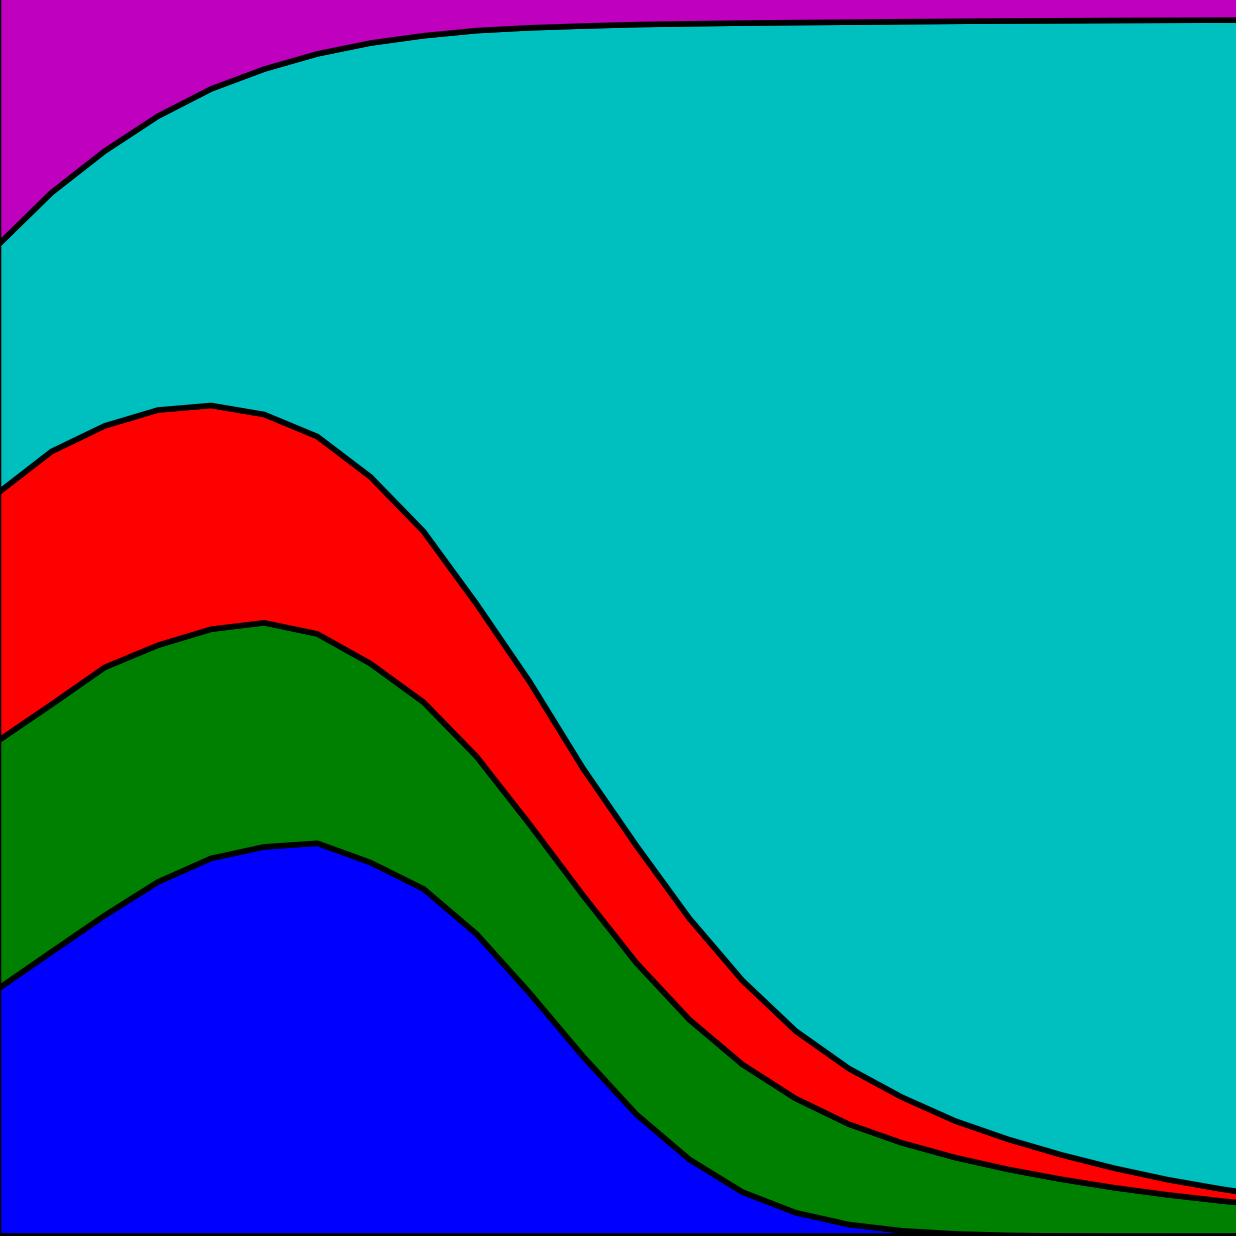
\includegraphics[width=0.24\textwidth]{static/axelrod-logo.png}
    \end{center}
\end{frame}

% \begin{frame}
%     \centering
%     \includestandalone[width=.85\textwidth]{static/game}
% \end{frame}

\begin{frame}
    \begin{center}
    \huge{
        \begin{equation*}
            \begin{pmatrix}
                (3, 3) & (0, 5) \\[6pt]
                (5, 0) & (1, 1)
            \end{pmatrix}
        \end{equation*}}
    \end{center}
\end{frame}

\begin{frame}
    \begin{center}
    \includestandalone[width=\textwidth]{static/iterated_prisoners_dilemma}
    \end{center}
\end{frame}

% \begin{frame}
%     \centering
%     \includestandalone[width=\textwidth]{static/tft_vs_defector}
% \end{frame}

% \begin{frame}
%     \centering
%     \includestandalone[width=\textwidth]{static/tft_vs_cooperator}
% \end{frame}

% \begin{frame}[fragile]
% 	\begin{minted}
%     [
%     framesep=4mm,
%     baselinestretch=1.2,
%     fontsize=\footnotesize,
%     ]
%     {python}
% class TitForTat(Player):
%     """A player starts by cooperating and then mimics previous
%     move by opponent."""

%     name = 'Tit For Tat'
%     classifier = {
%         'memory_depth': 1,  # Four-Vector = (1.,0.,1.,0.)
%         'stochastic': False,
%         'inspects_source': False,
%         'manipulates_source': False,
%         'manipulates_state': False
%     }

%     @staticmethod
%     def strategy(opponent):
%         return 'D' if opponent.history[-1:] == ['D'] else 'C'
%     \end{minted}
% \end{frame}

% \begin{frame}[fragile]
% 	\begin{minted}
%     [
%     framesep=4mm,
%     baselinestretch=1.2,
%     fontsize=\footnotesize,
%     ]
%     {python}
% class TestTitForTat(TestPlayer):

%     name = "Tit For Tat"
%     player = axelrod.TitForTat
%     expected_classifier = {
%         'memory_depth': 1,
%         'stochastic': False,
%         'inspects_source': False,
%         'manipulates_source': False,
%         'manipulates_state': False
%     }

%     def test_strategy(self):
%         """Starts by cooperating."""
%         self.first_play_test(C)
%     \end{minted}
% \end{frame}

\begin{frame}
    \centering
    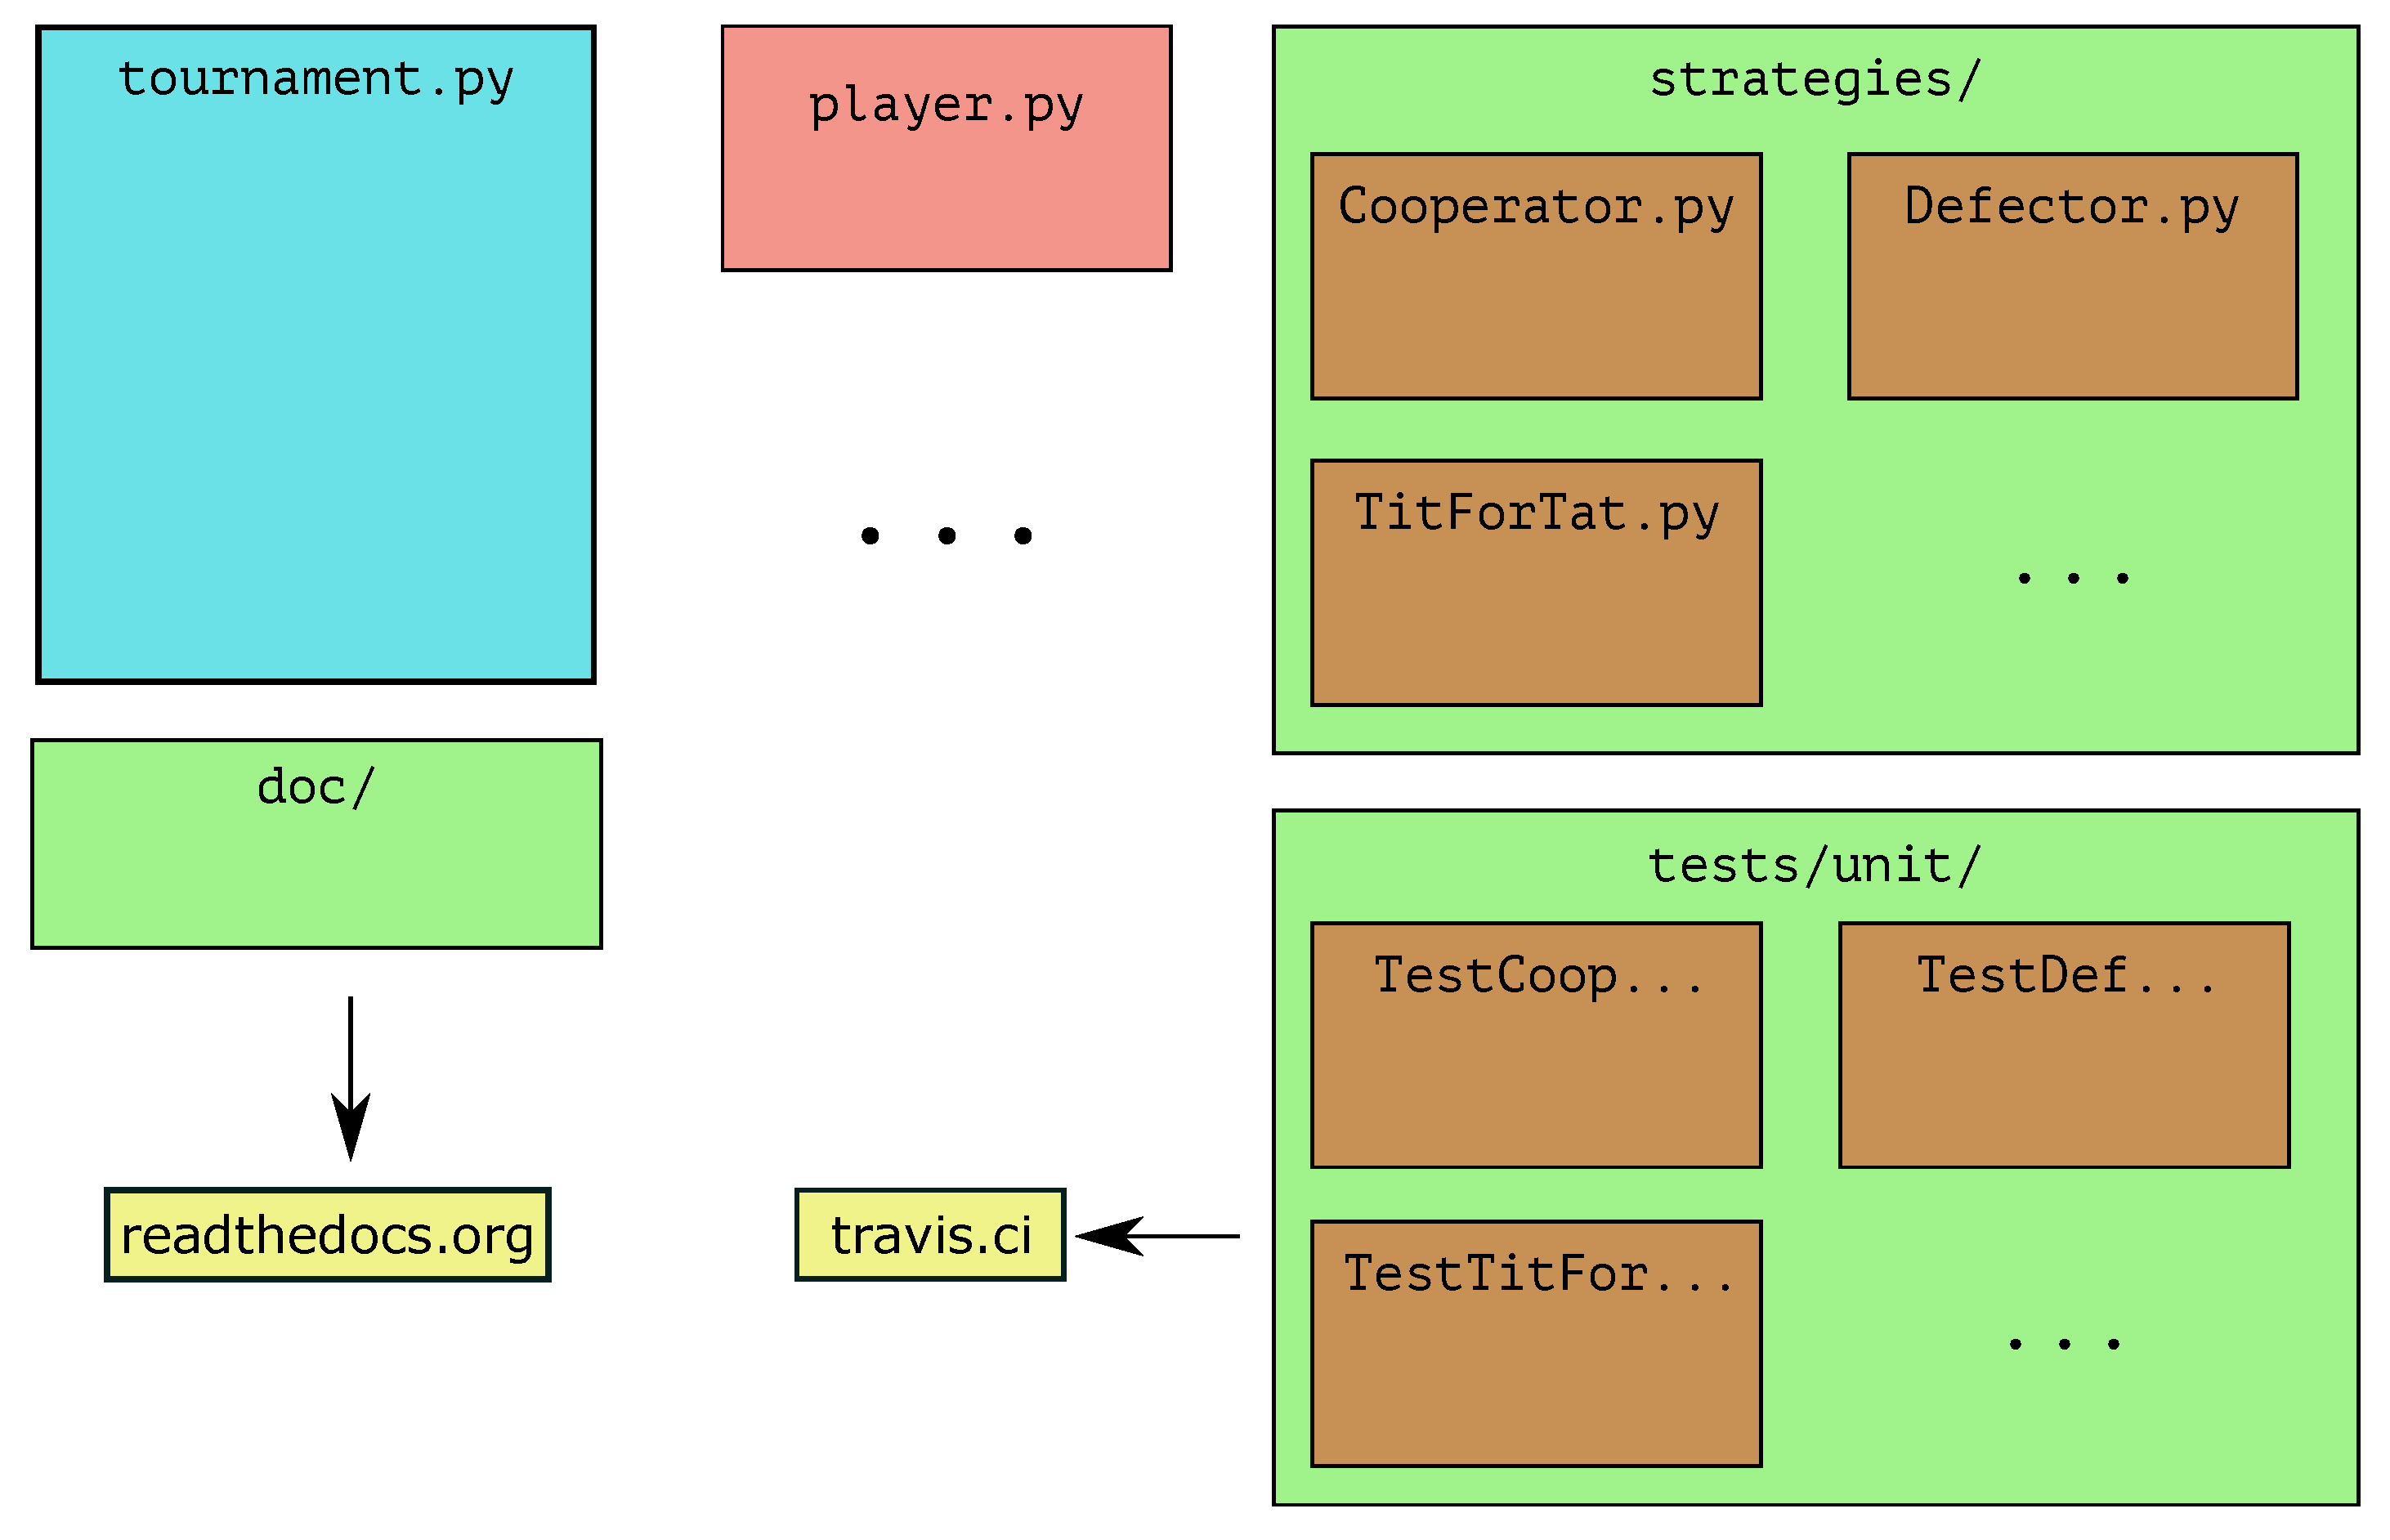
\includegraphics[width=\textwidth]{static/outline_of_library.pdf}
\end{frame}

% \begin{frame}
%     \centering
%     \Huge \textcolor{orange}{Research}
% \end{frame}


% \begin{frame}
%     \centering
%     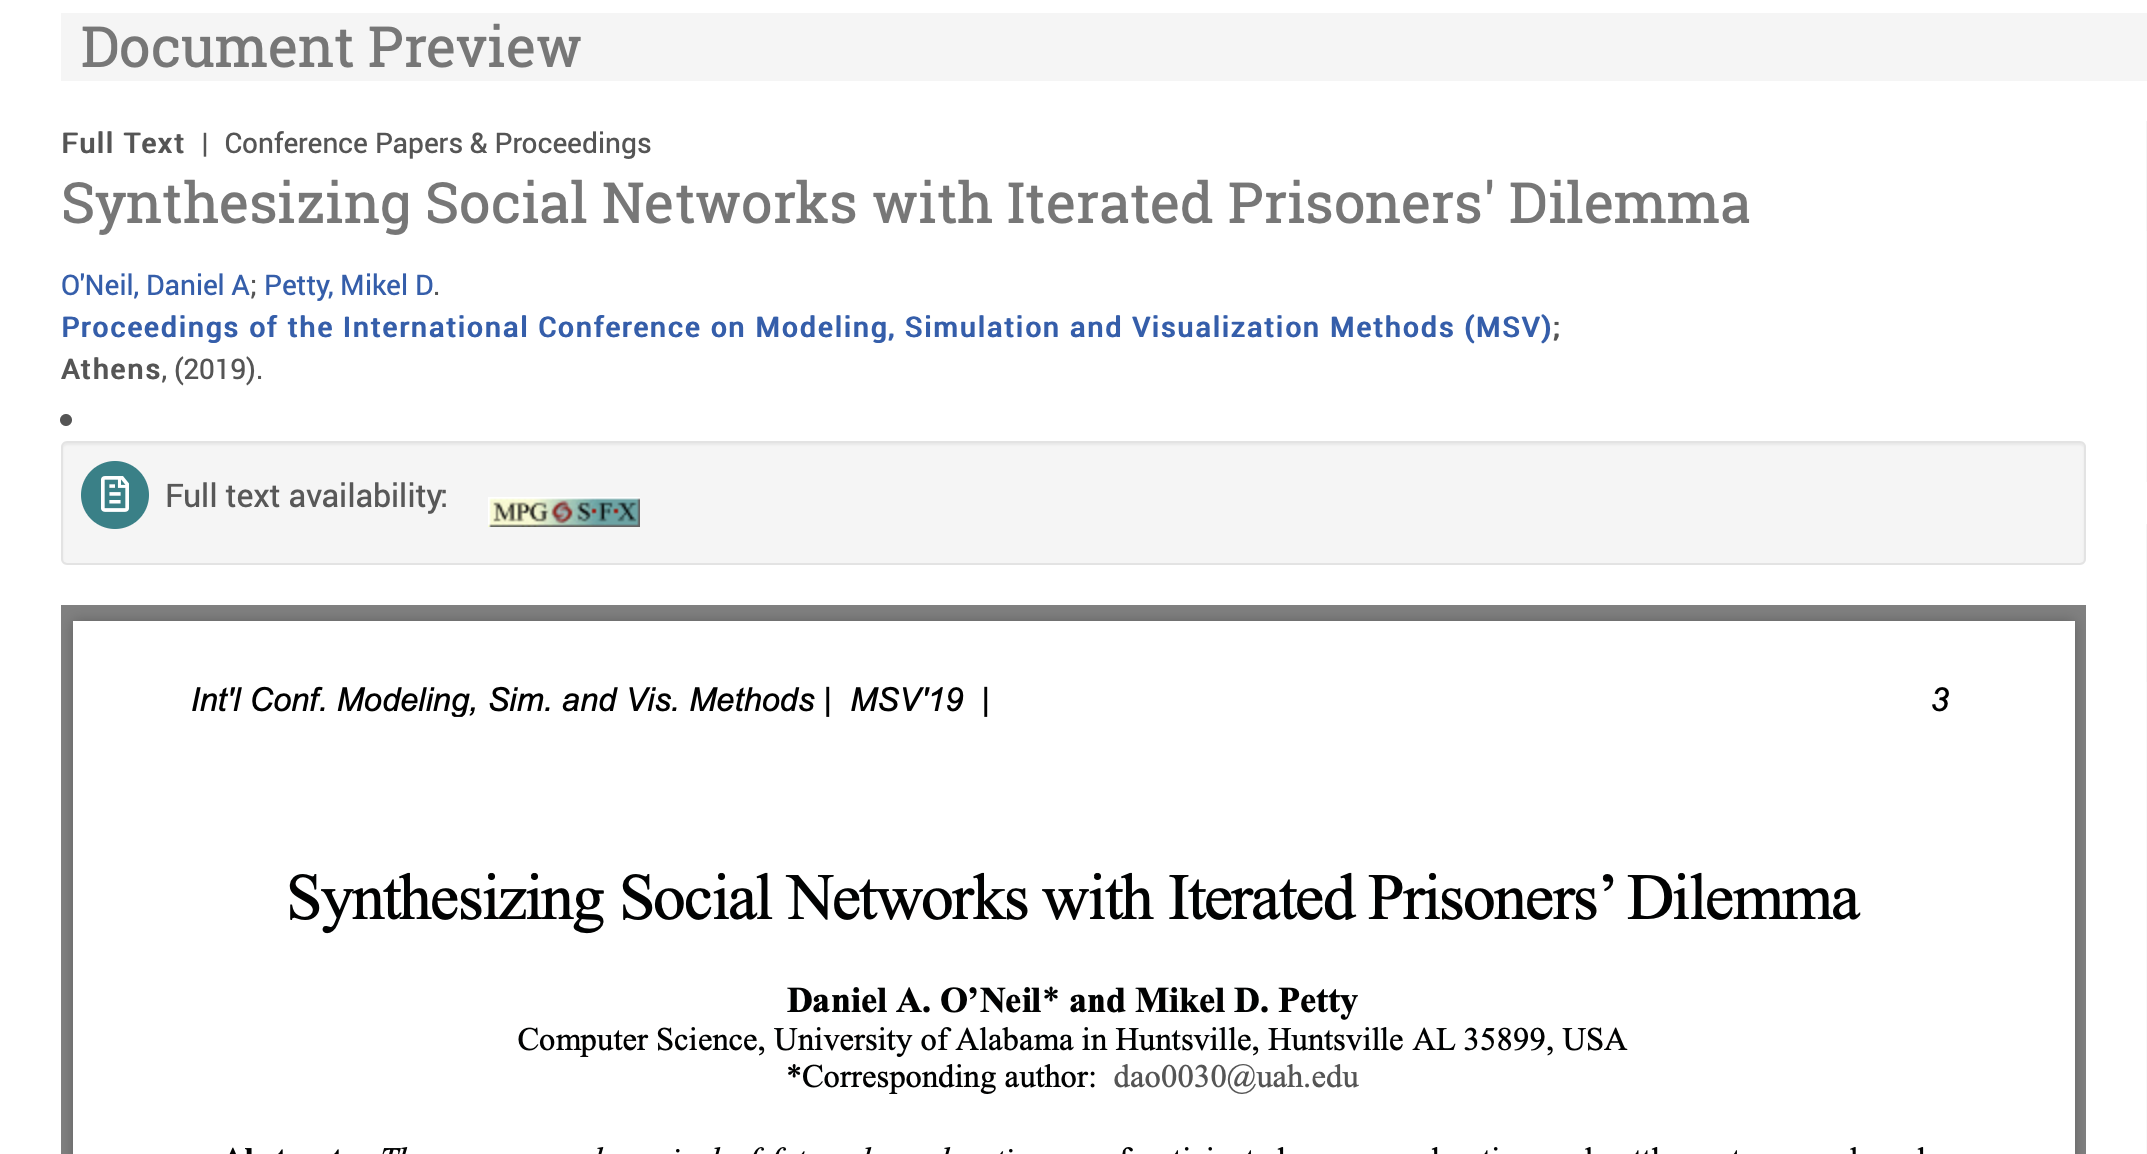
\includegraphics[width=.54\textwidth]{static/paper_one.png}\hspace{6pt}
%     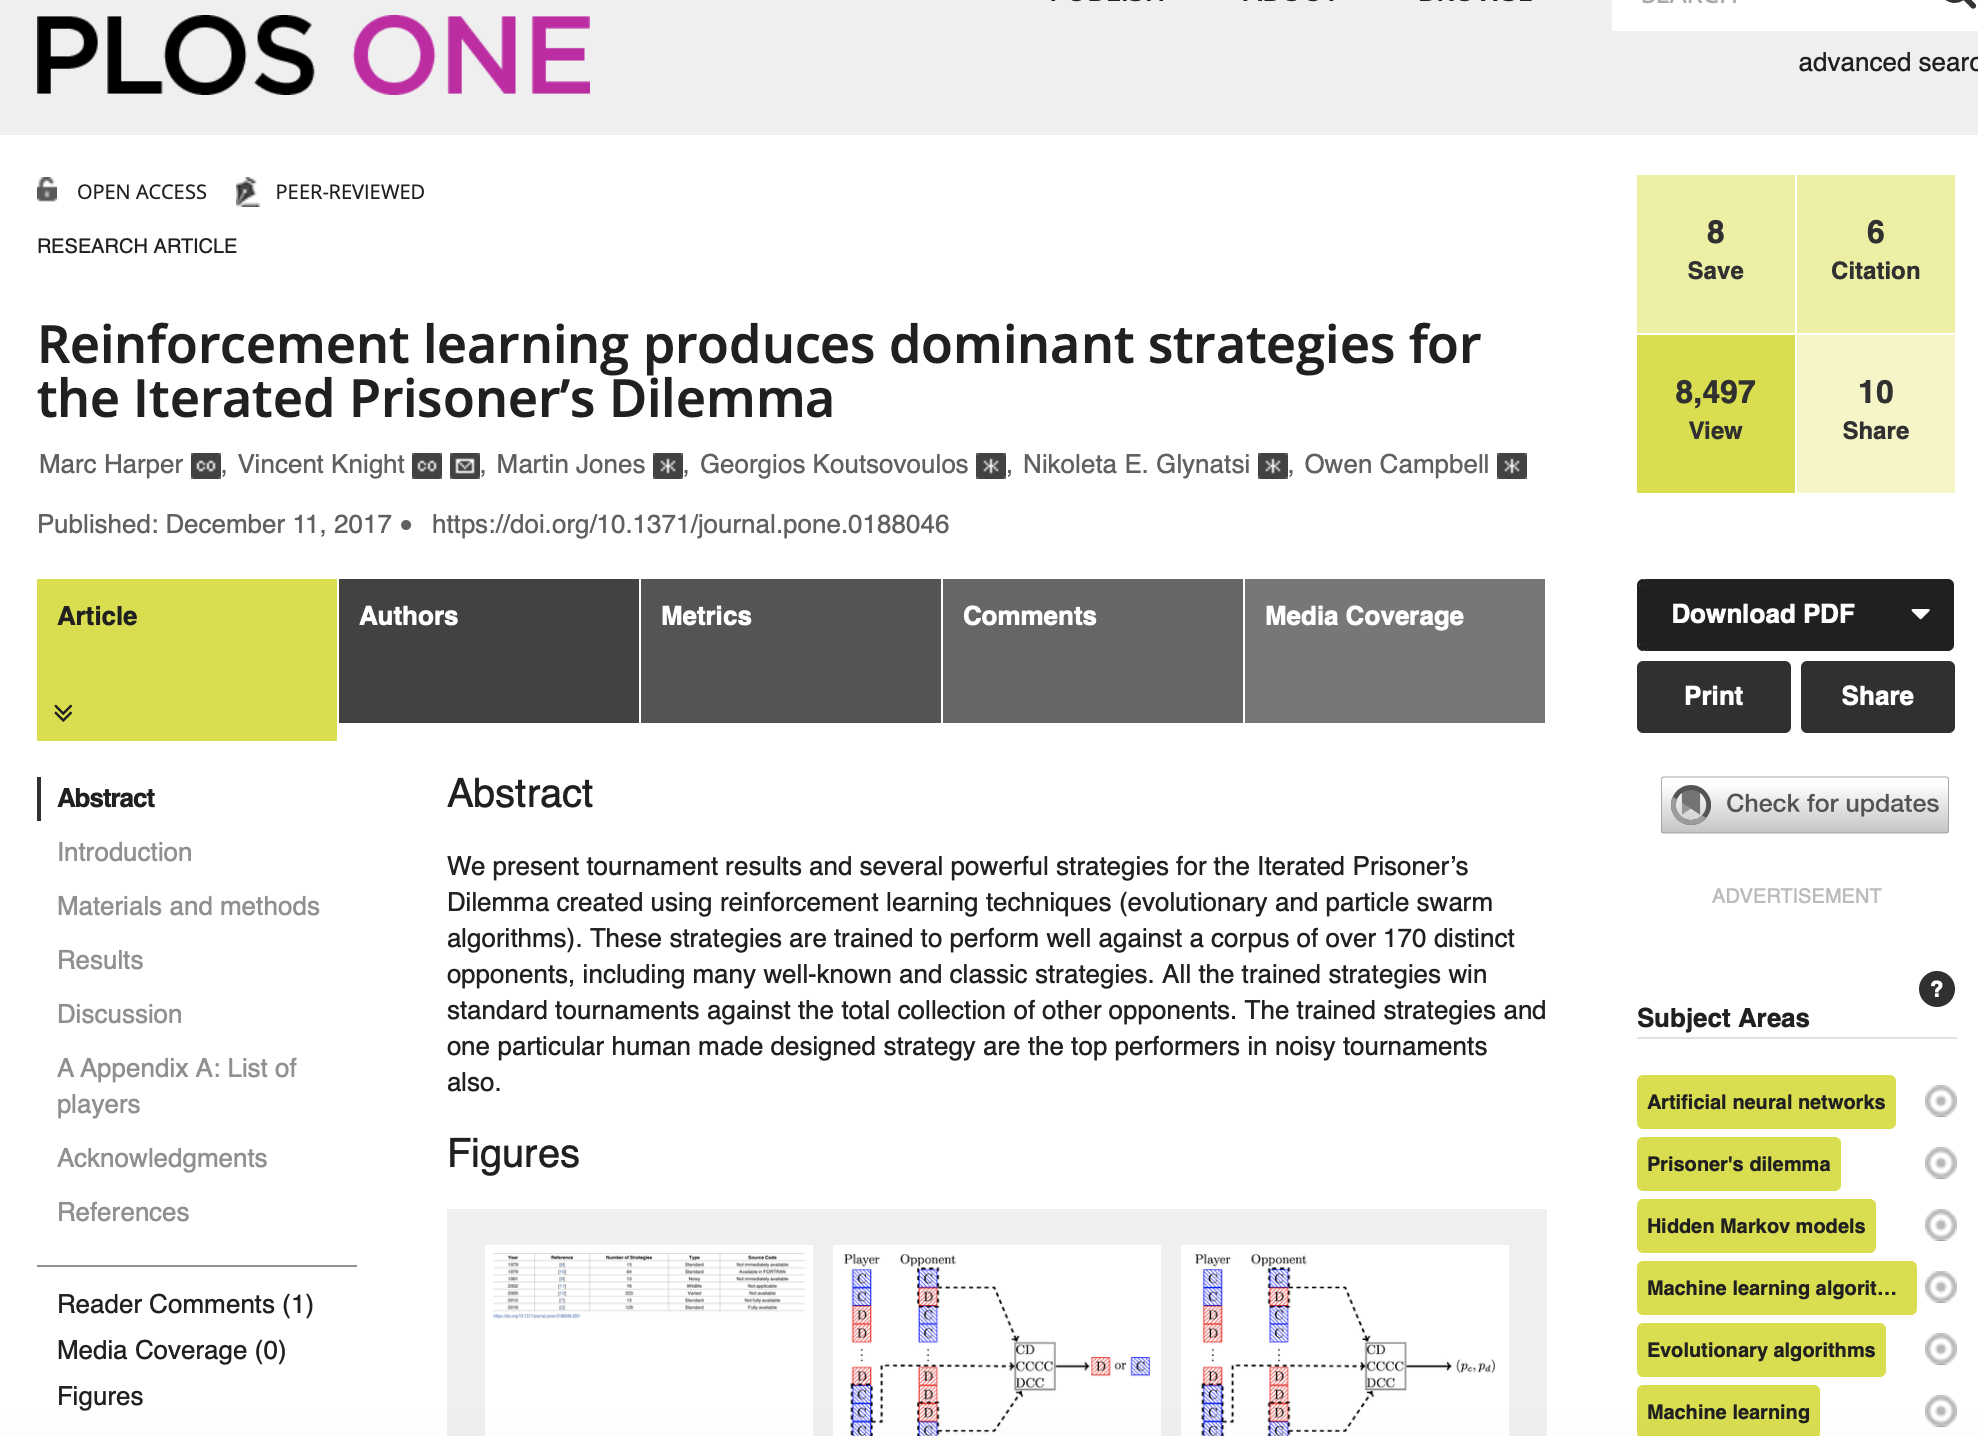
\includegraphics[width=.40\textwidth]{static/paper_two.png}\vfill

%     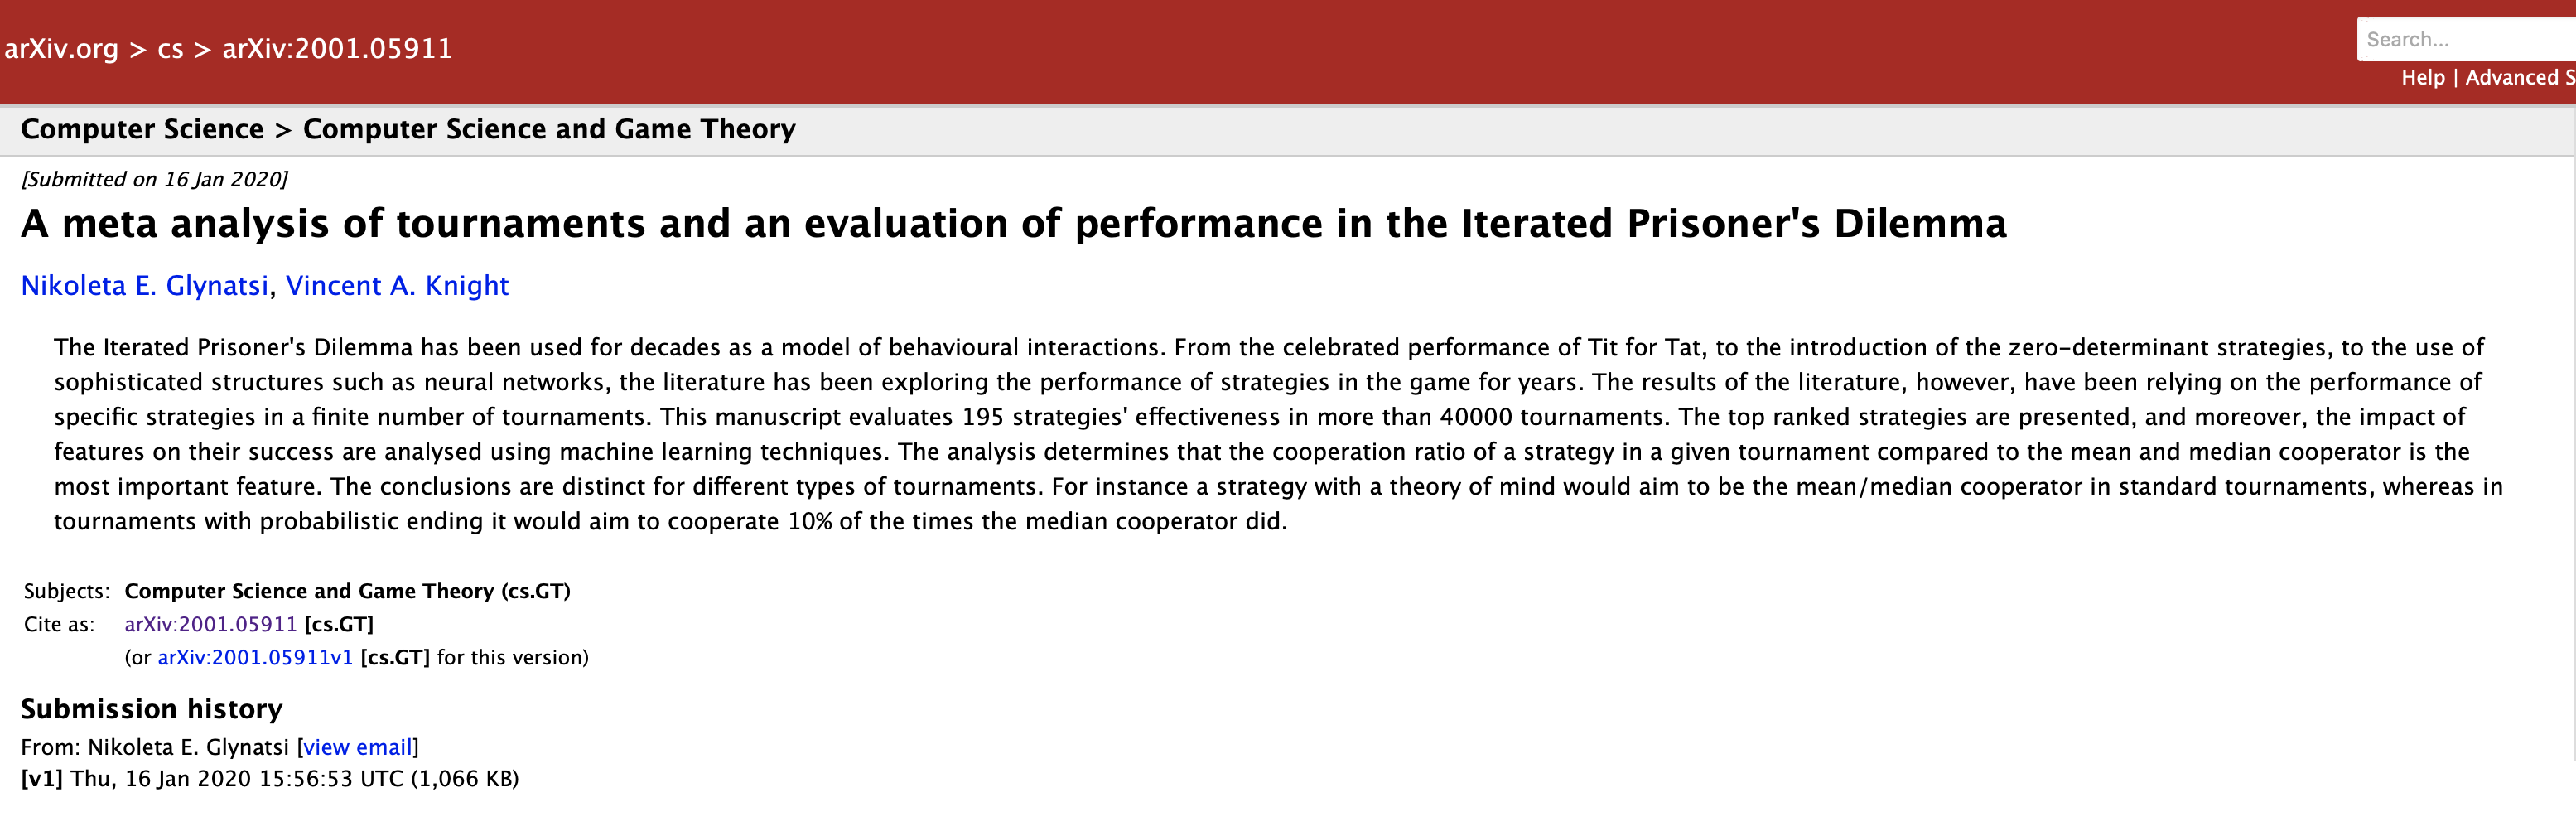
\includegraphics[width=.95\textwidth]{static/paper_three.png}
% \end{frame}

% \begin{frame}
%     \centering
%     \Huge \textcolor{orange}{Contributions}
% \end{frame}

\begin{frame}
    \centering
    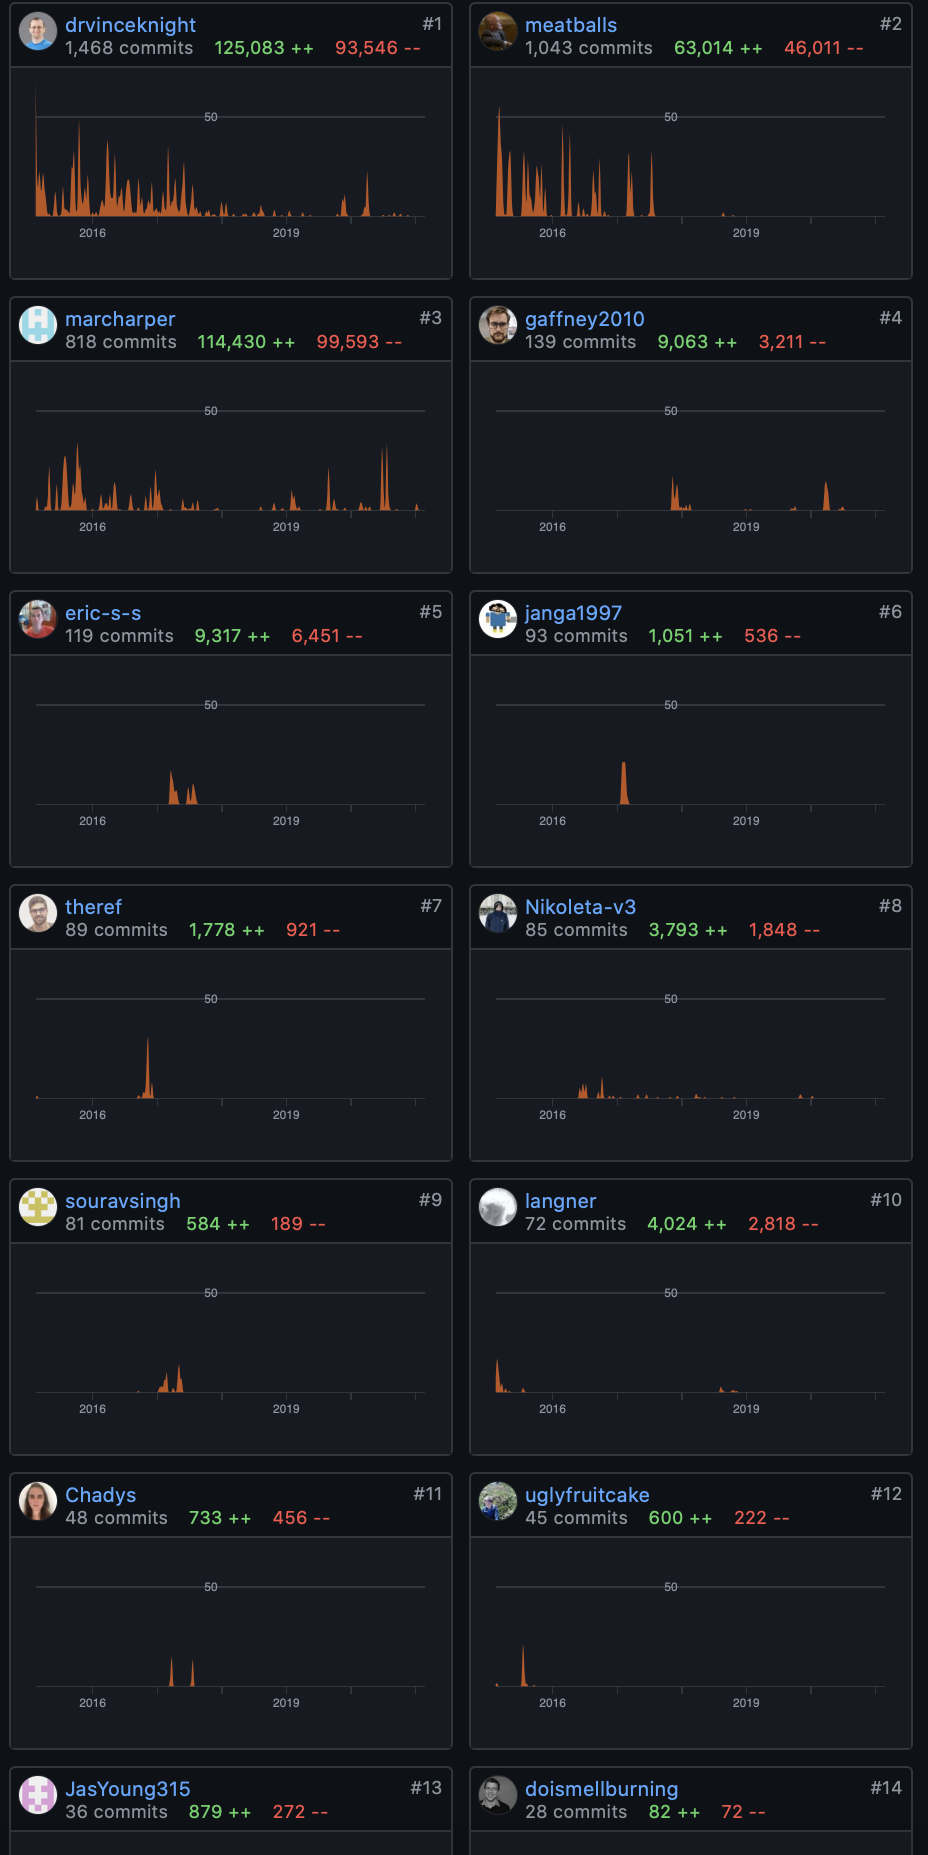
\includegraphics[width=.40\textwidth]{static/contributions.png}
\end{frame}

\begin{frame}
    \footnotesize
    ``And I really wanted to thank you all, I discovered your project because of a
    course where we needed to participate in an open source project, and I had
    the occasion to compare the welcome me and my coworkers received here
    compared to other people from my class who worked on different project. And
    I’ve got to said you are awesome on that part and on the help your provide
    to newbies I like your project so I’ll try to continue to contribute now and
    then!'' \\

    Julie Rymer - @Chadys -10 May 2017
\end{frame}

\begin{frame}
    \begin{center}
        \small
    \#ChooseToChallenge \\
    \faTwitter \ @NikoletaGlyn \\
    \faTwitter \ @AxelrodPython \\
    
    \vspace{1cm}
    \end{center}

    \footnotesize
    \faGithub \ \url{https://github.com/Axelrod-Python/Axelrod} \\
    $\bullet$ \url{https://axelrod.readthedocs.io/} \\
    $\bullet$ \url{https://axelrod.readthedocs.io/en/latest/tutorials/contributing/index.html} \\

    \faGithub  \ \url{https://github.com/drvinceknight} \\
    \faGithub  \ \url{https://github.com/gaffney2010} \\
    \faGithub  \ \url{https://github.com/marcharper} \\
    \faGithub  \ \url{https://github.com/meatballs} \\
\end{frame}

\begin{frame}
    \centering
    
\includegraphics[width=\textwidth]{static/my_first_pr.png}
\end{frame}
\end{document}